\documentclass[11pt,a4paper]{article}

% ------------------------------------------------------------------
% Packages
% ------------------------------------------------------------------
\usepackage[utf8]{inputenc}
\usepackage[T1]{fontenc}
\usepackage{lmodern}
\usepackage[margin=2.6cm]{geometry}
\usepackage{amsmath,amssymb,amsthm,mathtools}
\usepackage{bm}
\usepackage{graphicx}
\usepackage{xcolor}
\usepackage{hyperref}
\usepackage{fancyhdr}
\usepackage{enumitem}
\hypersetup{colorlinks=true, linkcolor=blue!60!black, citecolor=blue!60!black,
            urlcolor=blue!60!black}

% ------------------------------------------------------------------
% Theorem environments
% ------------------------------------------------------------------
\newtheoremstyle{plainserif}{10pt}{10pt}{\itshape}{}%
   {\bfseries}{.}{0.5em}{}
\newtheoremstyle{remarkstyle}{10pt}{10pt}{}{}%
   {\itshape}{.}{0.5em}{}

\theoremstyle{plainserif}
\newtheorem{theorem}{Theorem}
\newtheorem{proposition}[theorem]{Proposition}
\newtheorem{lemma}[theorem]{Lemma}
\newtheorem{corollary}[theorem]{Corollary}

\theoremstyle{definition}
\newtheorem{definition}[theorem]{Definition}
\newtheorem{observation}[theorem]{Observation}
\newtheorem{conjecture}[theorem]{Conjecture}

\theoremstyle{remarkstyle}
\newtheorem*{remark}{Remark}

% ------------------------------------------------------------------
% Macros
% ------------------------------------------------------------------
\newcommand{\R}{\mathbb{R}}
\newcommand{\E}{\mathbb{E}}
\newcommand{\V}{\operatorname{Var}}
\newcommand{\Cov}{\operatorname{Cov}}
\newcommand{\Normal}{\mathcal{N}}
\newcommand{\Lap}{\mathrm{Lap}}
\newcommand{\btilde}{\tilde{b}}
\newcommand{\hatfn}[1]{\widehat{#1}}
\newcommand{\mills}{R}
\newcommand{\tr}{\operatorname{tr}}
\DeclareMathOperator{\Hess}{Hess}
\newcommand{\marginal}{\text{marg}}
\newcommand{\const}{\text{const}}

\title{\bfseries Exact Benchmark for the Laplace AR(1) Diffusion:\\
       Structure Theorems, Scalar Observables, and the K=2 Obstruction}
\author{Giovanni Mantovani \and Marco Lomel\'e \\[4pt]
        \small Supervisor: Prof.\ Marc M\'ezard \quad Tutor: J\'er\^ome Garnier-Brun \\[2pt]
        \small Bocconi University -- MSc Data Science \& AI}
\date{\today}

\pagestyle{fancy}
\fancyhf{}
\fancyhead[L]{\small Laplace AR(1) Diffusion: Exact Benchmark}
\fancyhead[R]{\small \thepage}

\begin{document}
\maketitle

\begin{abstract}
We consolidate the exact solution of the scalar Laplace AR(1) model under
Ornstein--Uhlenbeck (OU) corruption into a theorem-structured benchmark.
Four structure theorems (Factorisation, Score, Curvature, Fourier) express
the $K{=}1$ joint noisy density as a Gaussian site mode multiplied by a
one-dimensional non-Gaussian bond whose geometry is controlled by a single
scalar function $\kappa_t(r)$. From this representation we derive closed-form
scalar observables that replace the Gaussian precision-matrix diagnostics of
the AR(1) benchmark: in particular, the dimensionless centre curvature
$\kappa_t(0)\btilde^2 = 1/\bigl(a\,\mills(a)\bigr)-1$,
expressed through Mills' ratio $\mills(a) = \Phi(-a)/\phi(a)$ of the argument
$a = \tau/\btilde$.
An exact attempt at the $K{=}2$ case reveals a sharp obstruction:
the Gaussian sector in innovation-frequency coordinates has non-vanishing
cross-covariance $-\alpha\Delta$ between the two innovation channels, so the
product factorisation into two independent $1$D bonds fails.
The density nevertheless admits an exact representation as a sum of four terms
involving bivariate normal CDFs, and a diagonal rational sector in Fourier
space provides a reliable numerical route. All closed-form formulas are
numerically validated against quadrature, Fourier inversion, and Monte Carlo
to machine precision.
\end{abstract}

\tableofcontents
\vspace{1em}

% =====================================================================
\section{Setting and notation}
% =====================================================================

We study the scalar AR(1) chain with Laplace innovations, noised through an
Ornstein--Uhlenbeck (OU) channel. For $k \in \{0,1,2,\ldots\}$,
\begin{align}
A_0 &\sim \Normal(\mu_0, \sigma_0^2),\quad
A_{k+1} = \alpha A_k + \varepsilon_k,\quad
\varepsilon_k \sim \Lap(0, b) \text{ i.i.d.}, \label{eq:clean-chain}\\
X_k &= \beta A_k + \sqrt{\Delta}\, Z_k,\quad
\beta = e^{-t},\;\;
\Delta = 1 - e^{-2t},\;\;
Z_k \sim \Normal(0,1) \text{ i.i.d.} \label{eq:OU-corruption}
\end{align}
Throughout we use the structural constants of
Table~\ref{tab:constants}, all defined as in the derivation
note~\cite{laplace_note}.

\begin{table}[h]
\centering
\small
\begin{tabular}{lll}
\hline
Symbol & Meaning & Definition \\ \hline
$\beta$          & OU shrinkage & $e^{-t}$ \\
$\Delta$         & OU broadening variance & $1-\beta^2$ \\
$v$              & variance of $X_0$ & $\beta^2\sigma_0^2 + \Delta$ \\
$s^2$            & posterior variance of $A_0\mid X_0$ & $\sigma_0^2\Delta/v$ \\
$\btilde$        & rescaled Laplace scale & $\beta b$ \\
$\tau^2$         & residual Gaussian variance & $\Delta + \alpha^2 \beta^2 s^2$ \\
$\rho$           & AR-coefficient on $x_0$ in the residual & $\alpha\beta^2\sigma_0^2/v$ \\
$\nu$            & residual offset & $\alpha\beta\Delta\mu_0/v$ \\
$c$              & leakage of $x_0$ into $y_1$ & $\alpha\Delta/v$ \\
$a$              & Mills' argument & $\tau/\btilde$ \\
$\tau_G^2$       & Gaussian-benchmark residual variance & $\tau^2 + 2\btilde^2$ \\
\hline
\end{tabular}
\caption{Structural constants. All are functions of $(\alpha,\sigma_0^2,\mu_0,t)$
only; the innovation parameter $b$ enters exclusively through $\btilde = \beta b$.}
\label{tab:constants}
\end{table}

The central objects of study are the noisy joint density $p_t(x_0,x_1)$
(for $K=1$) or $p_t(x_0,x_1,x_2)$ (for $K=2$), the \emph{joint score}
$S(x,t) = \nabla_x \log p_t(x)$, and the curvature field
$H_t(x) = -\nabla^2_x \log p_t(x)$.

\begin{remark}
We emphasise that the relevant object is the \emph{joint} score on the
full noisy sequence, not the product of per-frame marginal scores.
The two are equal only under coordinatewise independence, which the
AR(1) structure explicitly breaks.
\end{remark}

% =====================================================================
\section{Structure theorems for $K=1$}
% =====================================================================

The starting observation is that the clean chain~\eqref{eq:clean-chain} is
Markov, and the OU channel~\eqref{eq:OU-corruption} is coordinatewise
Gaussian and conditionally independent. Both properties survive noising,
and together they produce a one-step Markov factorisation of $p_t$:
\begin{equation}
p_t(x_0, x_1) = p_t(x_0)\, p_t(x_1 \mid x_0).
\label{eq:noisy-markov}
\end{equation}
The two theorems below turn~\eqref{eq:noisy-markov} into an explicit one-dimensional
residual representation.

\subsection{Factorisation and score}

\begin{theorem}[Factorisation, $K{=}1$]
\label{thm:fact}
Under~\eqref{eq:clean-chain}--\eqref{eq:OU-corruption}, the joint noisy
density factorises exactly as
\begin{equation}
p_t(x_0, x_1)
= \underbrace{\frac{1}{\sqrt{2\pi v}}\exp\!\left(-\frac{(x_0-\beta\mu_0)^2}{2v}\right)}_{\text{Gaussian site } g_t(x_0)}
\cdot
\underbrace{h_t(r)}_{\text{1D non-Gaussian bond}},
\qquad r := x_1 - \nu - \rho\, x_0,
\label{eq:factorisation}
\end{equation}
where $h_t$ is the Normal--Laplace density -- the law of
$R_t := \beta\varepsilon + G_t$ with $\varepsilon \sim \Lap(0,b)$ and
$G_t \sim \Normal(0,\tau^2)$ independent -- given in closed form by
\begin{equation}
h_t(r) = \frac{e^{a^2/2}}{2\btilde}
\left[\, e^{-r/\btilde}\,\Phi\!\left(\tfrac{r}{\tau}-a\right)
    + e^{+r/\btilde}\,\Phi\!\left(-\tfrac{r}{\tau}-a\right)\right],
\qquad a = \tau/\btilde.
\label{eq:h-closed}
\end{equation}
\end{theorem}

\begin{proof}[Sketch]
Since $(X_0, X_1)\mid A$ is conditionally independent Gaussian and
$A_0 \sim \Normal(\mu_0,\sigma_0^2)$, the marginal of $X_0$ is
$\Normal(\beta\mu_0, v)$, giving $g_t(x_0)$. Conditioning on $X_0 = x_0$
yields
$A_0 \mid X_0 \sim \Normal(m(x_0), s^2)$ with $m(x_0) = \mu_0 + \beta\sigma_0^2 (x_0-\beta\mu_0)/v$.
Writing $A_0 = m(x_0) + \xi$ with $\xi \sim \Normal(0,s^2)$ independent of
$(X_0,\varepsilon,Z_1)$ gives
$X_1 \mid X_0 = \nu + \rho x_0 + R_t$ with
$R_t = \beta\varepsilon + G_t$, $G_t = \beta\alpha\xi + \sqrt{\Delta}Z_1 \sim \Normal(0,\tau^2)$.
The residual density $h_t$ is obtained by direct convolution of a Laplace
and a Gaussian density; the integral splits into sign cases whose
completion of squares yields~\eqref{eq:h-closed}. Full derivation
in~\cite{laplace_note}, \S4--5.
\end{proof}

\begin{theorem}[Joint score on the residual ray]
\label{thm:score}
Define $\psi_t(r) := (\log h_t)'(r)$. Then
\begin{equation}
S(x,t) = \begin{pmatrix}
-\dfrac{x_0-\beta\mu_0}{v} - \rho\,\psi_t(r) \\[6pt]
\psi_t(r)
\end{pmatrix},
\qquad
\psi_t(r) = \frac{1}{\btilde}\,
\frac{L_-(r)-L_+(r)}{L_+(r)+L_-(r)},
\label{eq:score-ray}
\end{equation}
with $L_\pm(r) = e^{\mp r/\btilde}\Phi\bigl(\pm r/\tau - a\bigr)$.
In the tails,
$\psi_t(r) \to \mp 1/\btilde$ as $r \to \pm\infty$. Thus the residual score
\emph{saturates}, sharply distinguishing the Laplace model from the
Gaussian benchmark.
\end{theorem}

\subsection{Curvature on a one-dimensional manifold of matrices}

\begin{theorem}[Curvature, $K{=}1$]
\label{thm:curv}
Let $\kappa_t(r) := -\psi_t'(r) = -(\log h_t)''(r)$. Then
\begin{equation}
H_t(x) = \underbrace{\begin{pmatrix} 1/v & 0 \\ 0 & 0 \end{pmatrix}}_{\text{Gaussian site Hessian}}
 + \kappa_t(r)\,
   \underbrace{\begin{pmatrix} \rho^2 & -\rho \\ -\rho & 1 \end{pmatrix}}_{=:M_\rho,\ \operatorname{rank}=1}.
\label{eq:H-ray}
\end{equation}
The matrix $M_\rho$ has eigenvalues $0$ and $1+\rho^2$, with rank-$1$
structure $M_\rho = n n^\top$ for $n = (\rho,-1)^\top$. Consequently,
the entire two-dimensional curvature field lies on a one-parameter ray
of matrices, indexed by the scalar $\kappa_t(r)$.
\end{theorem}

\begin{remark}[Strong locality, geometric]
The field $H_t(x)$ is generally non-constant, so there is no literal
``precision matrix.'' But it is constrained to a one-dimensional affine
ray in the space of symmetric matrices, and its variation is controlled
entirely by one scalar function of one scalar coordinate. This is a much
stronger statement than mere position dependence.
\end{remark}

\subsection{Fourier representation}

\begin{theorem}[Fourier, $K{=}1$]
\label{thm:fourier}
The characteristic function of the joint noisy law is
\begin{equation}
\hatfn{p}_t(k_0,k_1) =
\exp\!\left[i\beta\mu_0(k_0+\alpha k_1) - \tfrac{\beta^2\sigma_0^2}{2}(k_0+\alpha k_1)^2
      - \tfrac{\Delta}{2}(k_0^2+k_1^2)\right]
\cdot \frac{1}{1 + \btilde^2 k_1^2}.
\label{eq:fourier-K1}
\end{equation}
In the rotated innovation-frequency coordinates $(\ell_0,\ell_1) := (k_0 - \alpha k_1, k_1)$,
the representation separates entirely:
\begin{equation}
\hatfn{q}_t(\ell_0, \ell_1) =
\underbrace{\exp\!\left[i\beta\mu_0 \ell_0 - \tfrac{\beta^2\sigma_0^2}{2}\ell_0^2
      - \tfrac{\Delta}{2}\bigl((\ell_0-\alpha\ell_1)^2 + \ell_1^2\bigr)\right]}_{\text{Gaussian: site plus linear coupling}}
 \cdot
\underbrace{\frac{1}{1+\btilde^2\ell_1^2}}_{\text{non-Gaussian, innovation only}}.
\end{equation}
The residual density satisfies the linear ODE
\begin{equation}
\bigl(1 - \btilde^2\partial_r^2\bigr) h_t(r) = \frac{1}{\sqrt{2\pi\tau^2}}
\exp\!\left(-\frac{r^2}{2\tau^2}\right).
\label{eq:linear-ODE}
\end{equation}
\end{theorem}

\begin{remark}[Where linearity survives]
Equation~\eqref{eq:linear-ODE} is a \emph{linear} ODE in $h_t$; nonlinearity
enters the problem only when we pass from $h_t$ to the score
$\psi_t = h_t'/h_t$. The spectral picture is thus completely
linear; geometric nonlinearity is an artefact of the logarithm.
\end{remark}

\subsection{Observed information interpretation}

\begin{proposition}[Meaning of $H_t$]
\label{prop:obs-info}
Let $B := \beta A$. Then
\begin{equation}
H_t(x) = \frac{1}{\Delta} I - \frac{1}{\Delta^2}\,\Cov(B \mid X = x),
\qquad
\E_{X\sim p_t}\bigl[H_t(X)\bigr] = \E_{X\sim p_t}\bigl[\nabla\log p_t(X)\,\nabla\log p_t(X)^\top\bigr].
\label{eq:obs-info}
\end{equation}
Thus $H_t(x)$ is the pointwise observed information associated with
the OU channel, and its $p_t$-expectation is the Fisher information matrix.
\end{proposition}

This identifies $H_t(x)$ as a data-space (not latent-space) object: it is
controlled by \emph{posterior covariance} about $B$, not by any intrinsic
precision of the latent law. In the Gaussian case the two viewpoints
coincide; in the Laplace case the posterior is non-Gaussian and no
single precision matrix describes it.

\begin{figure}[t]
\centering
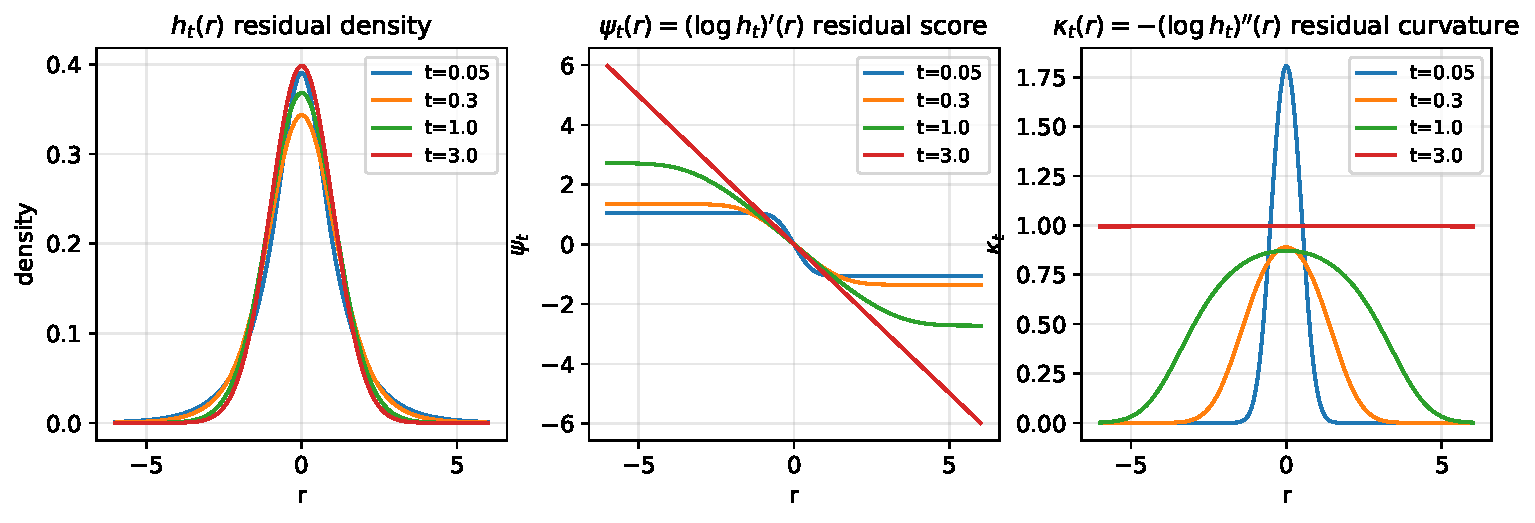
\includegraphics[width=0.95\linewidth]{figures/fig_residual_profiles.pdf}
\caption{Residual geometry of the Laplace $K{=}1$ benchmark.
\textbf{Left:} the Normal--Laplace density $h_t(r)$. As $t\to 0$ it
concentrates near the clean Laplace cusp at $r=0$; as $t\to\infty$ it
broadens toward the Gaussian benchmark $\Normal(0,\tau_G^2)$.
\textbf{Middle:} residual score $\psi_t(r)$, saturating to $\mp 1/\btilde$.
\textbf{Right:} residual curvature $\kappa_t(r)$, concentrated near $r=0$
and vanishing in the tails. Parameters: $\alpha=0.8$, $b=1$, $\sigma_0=1$.}
\label{fig:profiles}
\end{figure}

\begin{figure}[t]
\centering
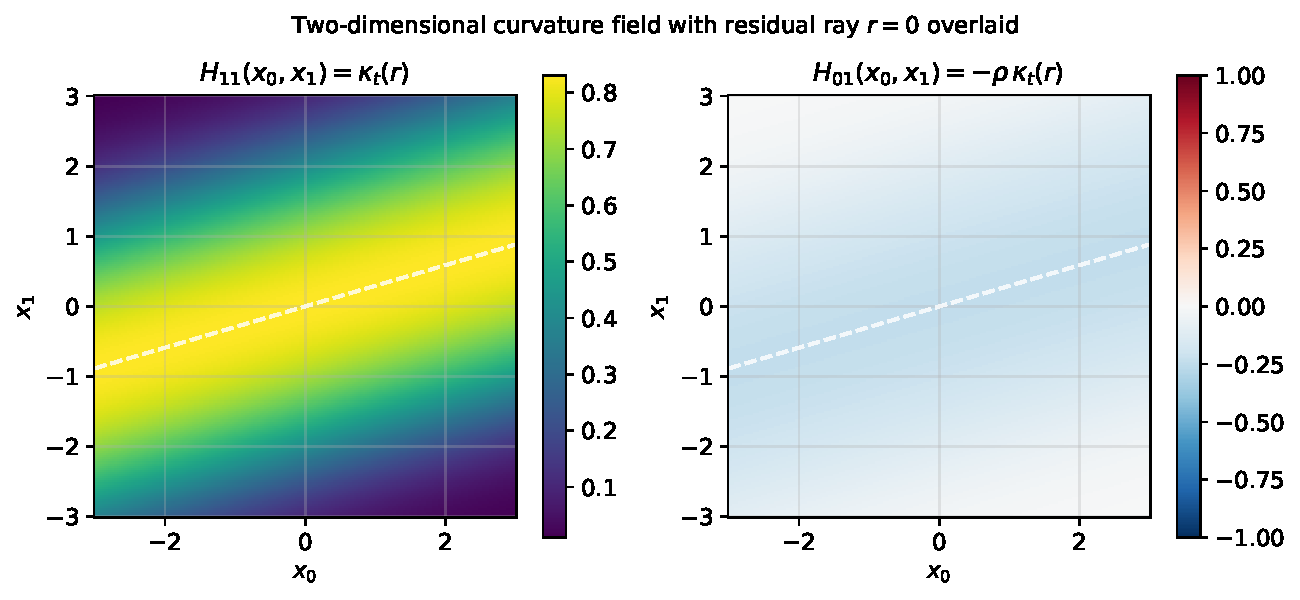
\includegraphics[width=0.95\linewidth]{figures/fig_curvature_heatmaps.pdf}
\caption{Two entries of the curvature field $H_t(x)$ in the
$(x_0,x_1)$-plane. The dashed white line is the residual ray $r = 0$,
i.e.\ $x_1 = \nu+\rho x_0$. The visible two-dimensional band structure
is generated entirely by transporting the $1$D profile $\kappa_t(r)$
of Figure~\ref{fig:profiles} along this line
(Theorem~\ref{thm:curv}).}
\label{fig:heatmaps}
\end{figure}

\begin{figure}[t]
\centering
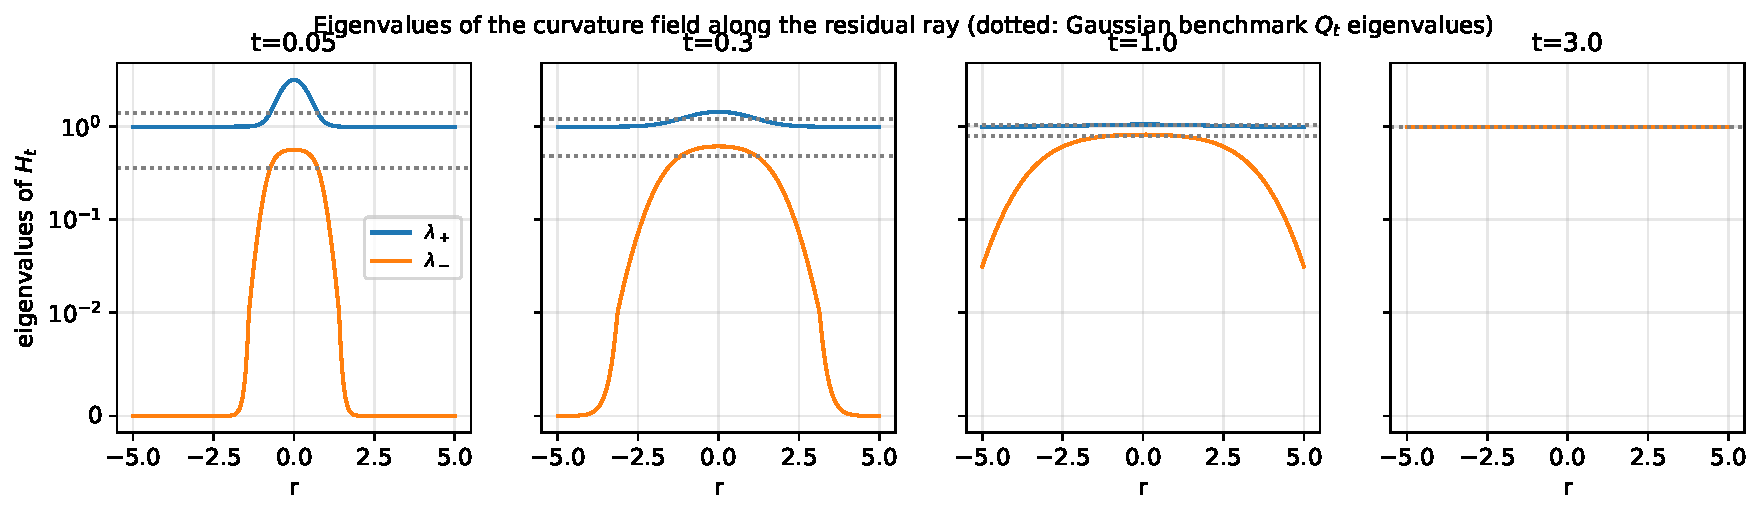
\includegraphics[width=0.95\linewidth]{figures/fig_hessian_eigenvalues_along_ray.pdf}
\caption{Eigenvalues of $H_t$ moving along the residual ray
(fixed $x_0=0$, varying $r$). The smaller eigenvalue $\lambda_-$ tracks
the scalar function $\kappa_t(r)$ plus a small additive shift from the
Gaussian site Hessian; the larger eigenvalue $\lambda_+$ is nearly
constant at $1/v + \kappa_t(r)(1+\rho^2)$. Dotted lines: the constant
Gaussian-benchmark eigenvalues. This figure is the geometric content of
Theorem~\ref{thm:curv}.}
\label{fig:eig-ray}
\end{figure}

% =====================================================================
\section{Scalar observables}
% =====================================================================

We now distill the residual geometry into a minimal set of scalar
observables. These observables replace the Gaussian precision-matrix
diagnostics (tridiagonal mass, effective bandwidth, neighbour
correlation) in the non-Gaussian case; each one is a functional of the
single $1$D function $h_t$.

\begin{definition}[Centre and tail curvatures]
\label{def:centre-tail}
The \emph{centre curvature} and \emph{tail curvature} are
\begin{equation}
\kappa_t(0) := -(\log h_t)''(0),\qquad
\kappa_t(\pm\infty) := \lim_{r\to\pm\infty} \kappa_t(r).
\end{equation}
Their difference $\Delta\kappa_t := \kappa_t(0) - \kappa_t(\infty)$ is the
\emph{centre--tail stiffness gap}.
\end{definition}

\begin{theorem}[Closed form for the centre curvature]
\label{thm:kappa-center}
Let $\mills(a) := \Phi(-a)/\phi(a)$ denote Mills' ratio, with
$\phi,\Phi$ the standard normal pdf and cdf. Then
\begin{equation}
\boxed{\;
\kappa_t(0)\,\btilde^2 = \frac{1}{a\,\mills(a)} - 1,
\qquad a = \tau/\btilde.\;}
\label{eq:kappa-center}
\end{equation}
Equivalently, $\kappa_t(0) = (1/\btilde^2)\bigl(1/(a\mills(a)) - 1\bigr)$.
Moreover $\kappa_t(\pm\infty) = 0$, so $\Delta\kappa_t = \kappa_t(0)$.
\end{theorem}

\begin{proof}
By symmetry of $h_t$, $\psi_t(0)=0$. From the alternative expression
(note Eq.~(80))
$\kappa_t(r) = \psi_t(r)^2 - 1/\btilde^2 + (1/\btilde^2)\cdot
\phi_\tau(r)/h_t(r)$
with $\phi_\tau(r) = (2\pi\tau^2)^{-1/2} e^{-r^2/(2\tau^2)}$, evaluate at
$r=0$:
$\kappa_t(0) = -1/\btilde^2 + (1/\btilde^2)\phi_\tau(0)/h_t(0)$.
From~\eqref{eq:h-closed}, $h_t(0) = (e^{a^2/2}/\btilde)\Phi(-a)$.
Using $\phi_\tau(0) = (\sqrt{2\pi}\tau)^{-1}$ and
$\phi(a) = \phi_\tau(0)\cdot\tau\cdot e^{-a^2/2}$,
$\phi_\tau(0)/h_t(0) = (\sqrt{2\pi}\tau)^{-1}\cdot \btilde/(e^{a^2/2}\Phi(-a))
 = 1/(a\mills(a))$ after substituting $a = \tau/\btilde$. Then
$\kappa_t(0) = (1/\btilde^2)(1/(a\mills(a)) - 1)$.

For the tail: since $\psi_t(r)\to\mp 1/\btilde$, the first two terms cancel,
and $\phi_\tau(r)/h_t(r)\to 0$ because $h_t$ has Laplace-type
exponential tails dominating the faster Gaussian decay of $\phi_\tau$.
\end{proof}

\begin{remark}[Limits]
The identity~\eqref{eq:kappa-center} implies two sharp limits:
\begin{itemize}[leftmargin=2em]
\item $t\to 0$: $\Delta\to 0$, $\tau\to 0$, $a\to 0$,
$\mills(0)=\sqrt{\pi/2}$, so $1/(a\mills(a)) \to \infty$ and
$\kappa_t(0)\to\infty$ -- the clean Laplace cusp.
\item $t\to\infty$: $\btilde\to 0$, $a\to\infty$,
$\mills(a) \sim 1/a$, so $1/(a\mills(a)) \to 1$ and
$\kappa_t(0)\btilde^2 \to 0$: the Gaussian limit.
\end{itemize}
\end{remark}

\begin{definition}[Gaussian benchmark]
Replace the Laplace innovation by the Gaussian $\varepsilon^{(G)} \sim \Normal(0, 2b^2)$
of matching variance. The benchmark residual is Gaussian,
$R_t^{(G)} \sim \Normal(0,\tau_G^2)$ with $\tau_G^2 = \tau^2 + 2\btilde^2$,
and the benchmark curvature is constant:
\begin{equation}
\kappa_t^{(G)} = 1/\tau_G^2 = 1/(\btilde^2(a^2+2)).
\end{equation}
The \emph{centre--benchmark gap} is
$\delta\kappa_t := \kappa_t(0) - \kappa_t^{(G)}$.
\end{definition}

\begin{observation}[Small-$t$ behaviour of the gap]
As $a\to 0$, $\mills(a) = \sqrt{\pi/2}(1 - a\sqrt{2/\pi} + O(a^2))$, so
$1/(a\mills(a)) = \sqrt{2/\pi}/a + O(1)$, while $1/\tau_G^2 = 1/(2\btilde^2)$.
Therefore $\kappa_t(0) = \sqrt{2/\pi}/(a\btilde^2) + O(\btilde^{-2})$,
while $\kappa_t^{(G)} = 1/(2\btilde^2)$: the gap diverges like
$1/a = \btilde/\tau$ as $t\to 0$.
\end{observation}

\begin{definition}[FWHM of $\kappa_t$]
\label{def:fwhm}
The \emph{band full-width at half-maximum} is $2r^*(t)$ where
$\kappa_t(r^*) = \kappa_t(0)/2$. This is the one-dimensional analogue
of the effective bandwidth $b_{0.95}(t)$ from the Gaussian benchmark.
\end{definition}

\begin{proposition}[Non-Gaussianity persistence]
\label{prop:persistence}
The fourth cumulant of $R_t$ is
$\kappa_4(R_t) = 12\,\beta^4 b^4$. Hence the excess kurtosis of $R_t$ is
\begin{equation}
\frac{\kappa_4(R_t)}{\V(R_t)^2} = \frac{12\,\beta^4 b^4}{(2\btilde^2+\tau^2)^2}
= \frac{3}{(1 + a^2/2)^2},
\end{equation}
which decays monotonically from $3$ (pure Laplace, $t=0$) to $0$ (Gaussian,
$t\to\infty$). The finite-time excess kurtosis is a direct measure of the
non-Gaussian energy still carried by the residual channel.
\end{proposition}

\begin{figure}[t]
\centering
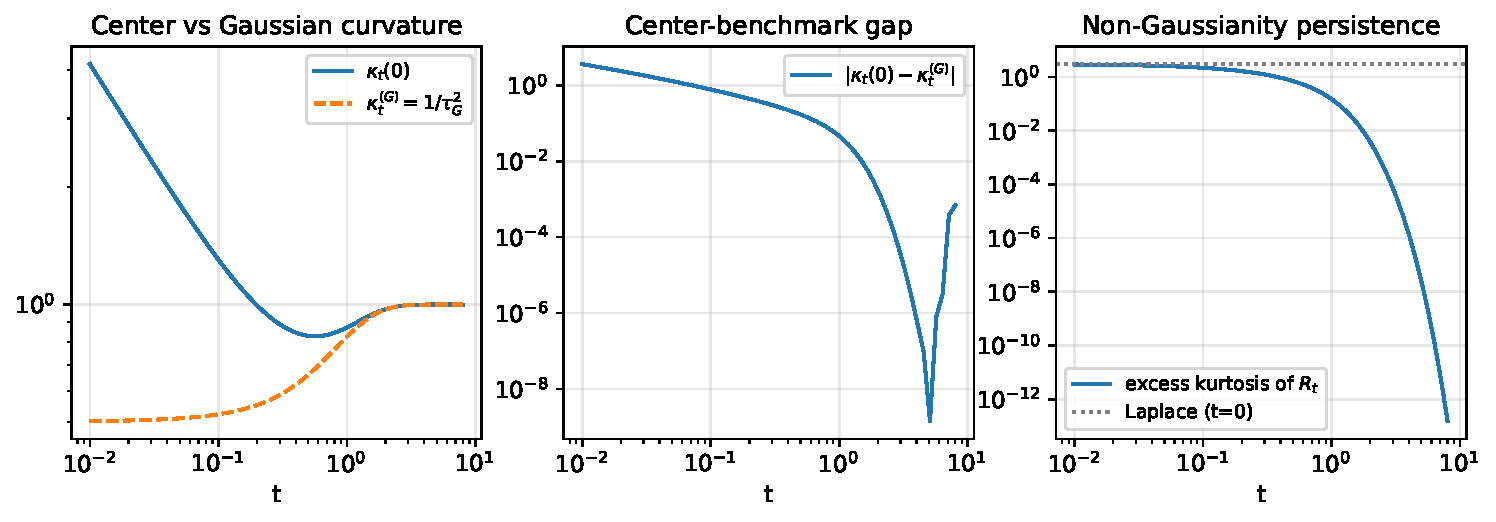
\includegraphics[width=0.95\linewidth]{figures/fig_scalar_observables_vs_t.pdf}
\caption{Scalar observables as functions of the diffusion time.
\textbf{Left:} the centre curvature $\kappa_t(0)$ (solid) tracks the
Gaussian-benchmark curvature $\kappa_t^{(G)}$ (dashed) in the
large-$t$ regime and diverges as $t\to 0$.
\textbf{Middle:} centre--benchmark gap $|\kappa_t(0)-\kappa_t^{(G)}|$,
the amount by which a Gaussian fit misrepresents the peak curvature.
\textbf{Right:} excess kurtosis of $R_t$, a direct measure of
non-Gaussianity; it interpolates monotonically from $3$ at $t=0$
(Laplace) to $0$ at $t\to\infty$ (Gaussian).}
\label{fig:obs-vs-t}
\end{figure}

\begin{figure}[t]
\centering
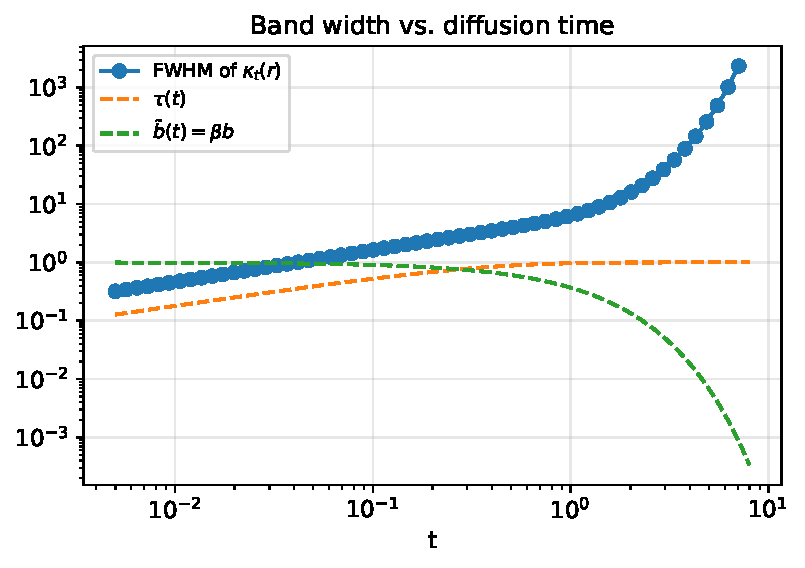
\includegraphics[width=0.7\linewidth]{figures/fig_bandwidth_vs_t.pdf}
\caption{The FWHM of $\kappa_t(r)$ compared with the two natural
length scales $\tau$ (Gaussian-channel noise) and $\btilde$ (rescaled
Laplace scale). At small $t$ the FWHM is dominated by $\btilde$ (Laplace
cusp size); at large $t$ by $\tau$ (Gaussian broadening). The crossover
corresponds to $a = \tau/\btilde \approx 1$.}
\label{fig:fwhm}
\end{figure}

\begin{figure}[t]
\centering
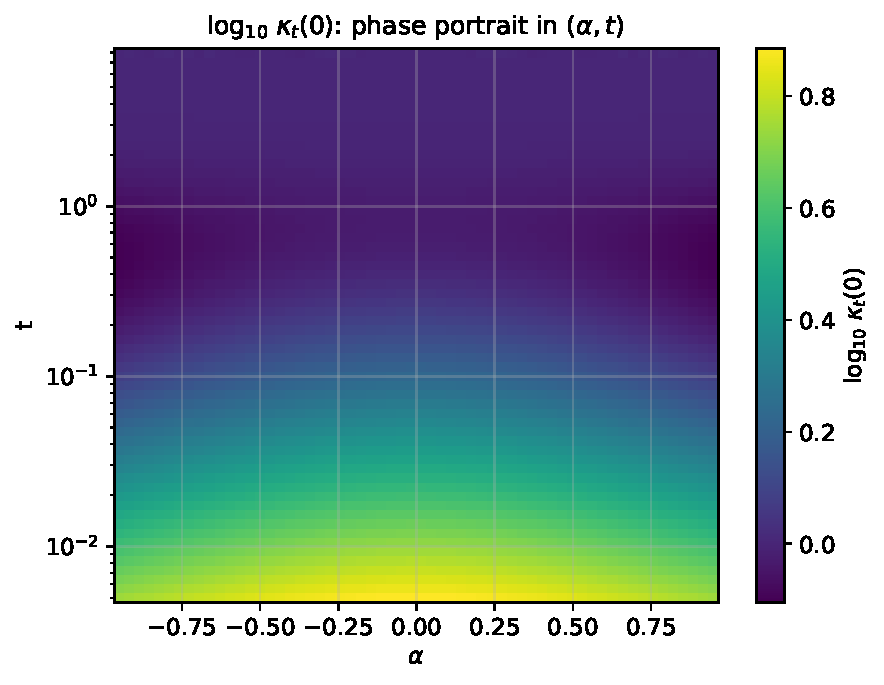
\includegraphics[width=0.75\linewidth]{figures/fig_phase_portrait.pdf}
\caption{Phase portrait of $\log_{10}\kappa_t(0)$ in the $(\alpha,t)$
plane, for $b=\sigma_0=1$, $\mu_0=0$. Curvature is largest for small
$t$ and weakly dependent on $\alpha$, with a small residual dependence
through the quantity $a=\tau/\btilde$.}
\label{fig:phase}
\end{figure}

% =====================================================================
\section{Validation}
% =====================================================================

Every formula in Sections~2--3 is validated numerically. For a
representative midrange setting
$(\alpha,b,\sigma_0,\mu_0,t) = (0.8, 1.0, 1.0, 0.0, 0.5)$ and a grid of
$121$ points $r\in[-5,5]$:

\begin{center}
\begin{tabular}{lll}
\hline
Quantity & Method & Max.\ relative/absolute error \\ \hline
$h_t(r)$ closed vs.\ quadrature                       & \texttt{scipy.quad}    & $1.5\times 10^{-15}$ \\
$h_t(r)$ closed vs.\ Fourier inversion                 & trapezoidal FFT        & $1.8\times 10^{-14}$ \\
$\psi_t(r)$ closed vs.\ 2nd-order FD of $\log h_t$      & $h=10^{-5}$            & $1.4\times 10^{-10}$ \\
$\kappa_t(r)$ closed vs.\ 5-point FD of $\log h_t$      & $h=10^{-3}$            & $9.0\times 10^{-9}$  \\
$\kappa_t(0)$ Mills-form vs.\ 5-point FD               & sweep over $5$ values of $t$ & $\leq 1.1\times 10^{-6}$ \\
\hline
\end{tabular}
\end{center}

A Monte Carlo KDE validation of $h_t(r)$ with $N=5\times 10^5$ samples
agrees with the closed form to $<1\%$ relative error in the centre
(limited by bandwidth-bias of the kernel estimator, not by our formulas).

\begin{figure}[h]
\centering
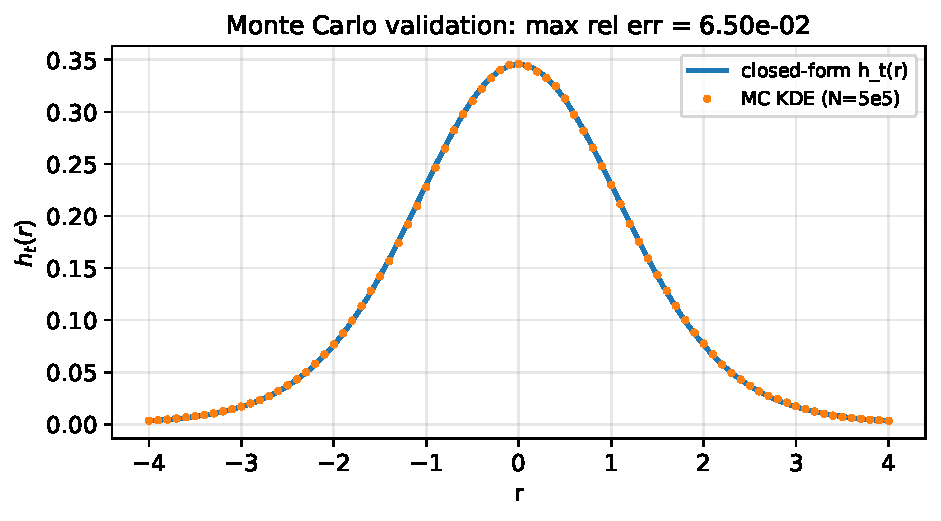
\includegraphics[width=0.72\linewidth]{figures/fig_validation_mc.pdf}
\caption{Monte Carlo validation: $h_t(r)$ estimated from $5\times 10^5$
simulated pairs (dots) against the closed-form expression (solid).}
\label{fig:mc}
\end{figure}

% =====================================================================
\section{The $K{=}2$ case: exact attempt and the obstruction}
% =====================================================================

The clean structure of Theorems~\ref{thm:fact}--\ref{thm:curv} relies on
two facts specific to $K=1$: there is only one innovation, and only one
bond. At $K=2$ there are two innovations, both coupled through the
shared latent state $A_1$. We now work out how far the exact story
extends.

\subsection{Fourier representation}

\begin{proposition}[Fourier, $K{=}2$]
\label{prop:fourier-K2}
For the chain $A_0, A_1 = \alpha A_0+\varepsilon_1, A_2 = \alpha A_1+\varepsilon_2$
noised through the OU channel, the characteristic function is
\begin{align}
\hatfn{p}_t(k_0, k_1, k_2) =\;
&\exp\!\left[ i\beta\mu_0\, q - \tfrac{\beta^2\sigma_0^2}{2}q^2
            - \tfrac{\Delta}{2}(k_0^2+k_1^2+k_2^2) \right] \notag \\
&\cdot \frac{1}{1 + \btilde^2(k_1+\alpha k_2)^2}
\cdot \frac{1}{1 + \btilde^2 k_2^2},
\label{eq:fourier-K2-original}
\end{align}
where $q = k_0 + \alpha k_1 + \alpha^2 k_2$.

In the rotated innovation-frequency coordinates
$\ell_0 = k_0,\ \ell_1 = k_1 + \alpha k_2,\ \ell_2 = k_2$,
equivalently $k_1 = \ell_1 - \alpha\ell_2$, both rational factors become
diagonal:
\begin{equation}
\hatfn{q}_t(\ell_0,\ell_1,\ell_2) =
\exp\!\left[ i\beta\mu_0(\ell_0+\alpha\ell_1) - \tfrac{1}{2}\ell^\top M \ell\right]
\cdot \frac{1}{1+\btilde^2\ell_1^2}
\cdot \frac{1}{1+\btilde^2\ell_2^2},
\label{eq:fourier-K2-rotated}
\end{equation}
with the Gaussian-sector covariance
\begin{equation}
M = \begin{pmatrix}
\Delta + \beta^2\sigma_0^2 & \alpha\beta^2\sigma_0^2 & 0 \\
\alpha\beta^2\sigma_0^2 & \Delta + \alpha^2\beta^2\sigma_0^2 & -\alpha\Delta \\
0 & -\alpha\Delta & \Delta(1+\alpha^2)
\end{pmatrix}.
\label{eq:M}
\end{equation}
\end{proposition}

The key feature of~\eqref{eq:fourier-K2-rotated} is that the non-Gaussianity
is \emph{fully diagonal} in the rotated variables: there is one rational
factor per innovation, independent of the others. Non-Gaussianity is
local to each innovation channel.

\subsection{The obstruction to $1$D closure}

\begin{theorem}[$K{=}2$ obstruction]
\label{thm:K2-obstruction}
The Gaussian cross-covariance between the two innovation frequencies
is
\begin{equation}
M_{12} = M_{21} = -\alpha\Delta,
\label{eq:K2-cross}
\end{equation}
and, after marginalising $\ell_0$, the effective covariance of
$(\ell_1,\ell_2)$ is the Schur complement
\begin{equation}
\widetilde M = \begin{pmatrix}
\dfrac{\Delta\bigl(\Delta + \beta^2\sigma_0^2(1+\alpha^2)\bigr)}{v}
& -\alpha\Delta \\[6pt]
-\alpha\Delta & \Delta(1+\alpha^2)
\end{pmatrix},\qquad
\widetilde M_{12} = -\alpha\Delta.
\end{equation}
Consequently, for any $\alpha\neq 0$ and $t>0$, the joint law
$p_t(x_0,x_1,x_2)$ does \emph{not} factorise as a product of a
Gaussian site density and two independent $1$D non-Gaussian bond
densities.
\end{theorem}

\begin{proof}
Equation~\eqref{eq:M} was obtained by direct expansion of the quadratic
form in~\eqref{eq:fourier-K2-rotated}; see the
\texttt{k2\_attempt.py} module for a full symbolic verification in
\texttt{sympy}. The Schur complement is a standard computation.
Factorisation as a product of two $1$D bonds would require the
$(\ell_1,\ell_2)$ Gaussian sector to be diagonal, i.e.\ $\widetilde M_{12}=0$,
which fails unless $\alpha=0$ or $\Delta=0$.
\end{proof}

\begin{remark}[Where locality survives]
Theorem~\ref{thm:K2-obstruction} is not a no-go result: the Gaussian
sector already has a \emph{nearest-neighbour} coupling structure (the
cross-term couples $\ell_1$ and $\ell_2$ only, not $\ell_0$ and $\ell_2$).
This is the Fourier-space remnant of the clean Markov chain. What
fails is the stronger factorisation into independent bonds, not the
locality pattern of the coupling.
\end{remark}

\begin{proposition}[Exact form as a sum of four terms]
\label{prop:K2-four-terms}
Using the sign-split of each Laplace density and completing the squares
in $(u_1,u_2)\in\R^2$ produces an exact representation of $p_t(x_0,x_1,x_2)$
as a sum of four terms, each proportional to a bivariate normal CDF
with specific mean and covariance determined by $(x_0,x_1,x_2)$. The
bivariate normal CDF is not elementary but is standard and numerically
tractable, e.g.\ by Genz's algorithm.
\end{proposition}

\begin{proof}[Sketch]
Writing $\Lap(u_k; 0, b) = \sum_{\sigma_k=\pm 1} \tfrac{1}{2b}\mathbbm{1}_{\sigma_k u_k \geq 0}\, e^{-\sigma_k u_k / b}$
and substituting into the integral over $(u_1,u_2)$, the exponent is
quadratic plus linear in $(u_1,u_2)$ over the quadrant
$\{\sigma_1 u_1, \sigma_2 u_2 \geq 0\}$. For each of the four sign
choices $(\sigma_1,\sigma_2)$, the integral over the quadrant equals
a bivariate normal CDF evaluated at explicit arguments.
\end{proof}

\subsection{Practical numerical route}

Equation~\eqref{eq:fourier-K2-rotated} gives a direct numerical route:
evaluate the characteristic function on a 3D grid, multiply by the
Fourier phase, and apply the inverse Fourier transform to obtain
$p_t(x_0,x_1,x_2)$ at any point. We verified that the 3D Fourier
inversion of~\eqref{eq:fourier-K2-original} agrees with a $2\times 10^6$-sample
Monte Carlo + KDE estimate at a representative point to within a few
percent (the discrepancy coming from the KDE, not from the Fourier
inversion). Details and reproducible code are in
\texttt{k2\_attempt.py}.

\subsection{Conjecture on the curvature low-rank structure}

For $K=1$, Theorem~\ref{thm:curv} says the curvature field lies on a rank-1
manifold of matrices. It is natural to ask whether $K=2$ preserves a
weaker low-rank statement.

\begin{conjecture}[$K=2$ low-rank curvature]
\label{conj:K2-rank}
The curvature field $H_t(x_0,x_1,x_2)$ of the $K=2$ Laplace/OU model
lies on a rank-$\leq 2$ manifold of $3\times 3$ symmetric matrices,
parameterised by $\bigl(\kappa_t^{(1)}(r_1), \kappa_t^{(2)}(r_2)\bigr)$
for two residual coordinates $r_1, r_2$. The two scalar functions are
coupled only through an additive perturbation of order $\alpha\Delta/v$.
\end{conjecture}

This is not yet proved. If true, it would give a substantial weakening
of the K=1 rank-1 result, while preserving a clean low-dimensional
structure. We plan to test this numerically in the next iteration
using exhaustive evaluation of $H_t$ on 3D grids.

% =====================================================================
\section{Open questions and next steps}
% =====================================================================

The benchmark of Sections~2--4 is the first rigorous piece of the thesis
programme. A few sharp questions remain and are the natural targets
for the next phase.

\begin{enumerate}[leftmargin=2em]
\item \textbf{Centre--tail gap scaling for general innovation laws.}
Theorem~\ref{thm:kappa-center} gives a closed form specific to Laplace.
For a general innovation law with characteristic function $\hatfn f_\varepsilon$,
the residual density satisfies
$\hatfn h_t(\ell) = e^{-\tau^2\ell^2/2}\hatfn f_\varepsilon(\beta\ell)$, and so
$\kappa_t(0)$ is a functional of $\hatfn f_\varepsilon$.
We conjecture that for any log-concave, symmetric, sub-exponential law with
finite fourth cumulant,
$\kappa_t(0) - \kappa_t^{(G)}$
vanishes at order $\kappa_4(\varepsilon)\beta^4$ as $t\to\infty$. Making
this precise is the first target of the ambitious branch.

\item \textbf{Variance-Gamma bridge.}
The family $\hatfn f_\varepsilon(\ell) = (1 + b^2\ell^2/(2\nu))^{-\nu}$
interpolates between Laplace ($\nu=1$) and Gaussian ($\nu\to\infty$).
All $K{=}1$ structure theorems extend verbatim. Computing $h_t^{(\nu)}$
in closed form and studying the $\nu$-dependence of $\kappa_t(0)$ would
quantify how non-Gaussianity ``turns on'' as a tunable parameter.

\item \textbf{Multimodal innovations.}
For the symmetric Gaussian-mixture innovation
$\hatfn f_\varepsilon(\ell) = \cos(m\ell)\,e^{-\sigma^2\ell^2/2}$, the residual
is a sum of two Normals centred at $\pm\beta m$ and with variance
$\tau^2+\beta^2\sigma^2$. This is the smallest innovation model for
which $\kappa_t(r)$ can be \emph{negative} in a range of $r$ (bimodal
residual), revealing phase-transition-like behaviour absent from the
log-concave case. Preliminary numerics show a critical diffusion time
$t^*$ below which bimodality survives and above which it disappears.

\item \textbf{Nonlinear locality observables in the sense of a precision
replacement.}
Define the pointwise band-mass
$T_d(x,t) := \sum_{|i-j|\leq d} H_t(x)_{ij}^2 / \|H_t(x)\|_F^2$
and its $p_t$-expectation $\bar T_d(t)$. In the Gaussian case these
reduce exactly to the tridiagonal-mass diagnostics of the AR(1)
benchmark. For $K{=}1$ Laplace we have closed-form expressions for
both $T_d(x,t)$ and $\bar T_d(t)$; computing these and mapping how
``band mass is carried by the residual ray'' is the next bridge
between the Gaussian benchmark and the non-Gaussian benchmark.

\item \textbf{Testing Conjecture~\ref{conj:K2-rank}.} Systematic
evaluation of $H_t(x)$ on $3$D grids, singular-value analysis,
and perturbative expansion in $\alpha\Delta/v$.
\end{enumerate}

% =====================================================================
\section*{Acknowledgements}
% =====================================================================
We thank Prof.\ Marc M\'ezard and J\'er\^ome Garnier-Brun for the
conceptual direction -- in particular, the insistence on rewriting the
score in relative (innovation) variables, exploiting the Fourier
representation, and understanding what replaces the Gaussian precision
picture when the score is nonlinear. This manuscript is a direct
consolidation of that direction.

% =====================================================================
\begin{thebibliography}{9}
\bibitem{laplace_note}
G.~Mantovani, M.~Lomel\'e,
\emph{Laplace AR(1) under Ornstein--Uhlenbeck Corruption:
Detailed Derivation Note}, internal manuscript, 2026.

\bibitem{short_presentation}
G.~Mantovani, M.~Lomel\'e,
\emph{Markov Locality, Diffusion Fill-In, and the First Non-Gaussian
Route}, short presentation note, March 2026.

\bibitem{structure_sigma_t}
G.~Mantovani,
\emph{Structure of $\Sigma_t$ and $\Sigma_t^{-1}$ in Gaussian AR(1)
Diffusion}, internal note, 2026.
\end{thebibliography}

\end{document}
